\documentclass[dvisvgm,tikz]{standalone}
\begin{document}
  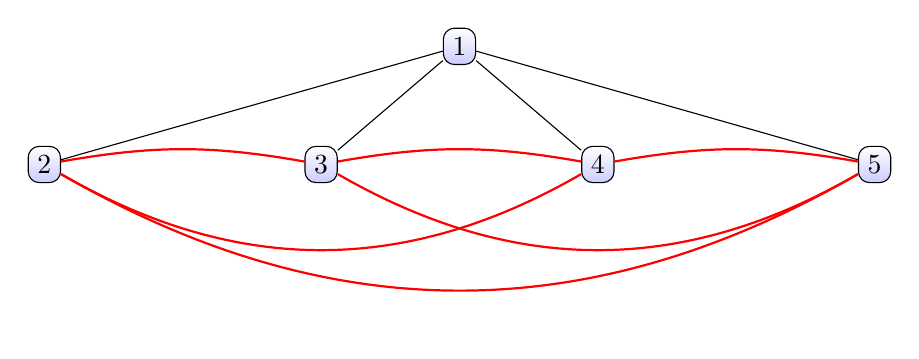
\begin{tikzpicture}[sibling distance=10em,
    every node/.style = {shape=rectangle, rounded corners,
    draw, align=center, top color=white, bottom color=blue!20}]
    \node (n1) {1}
      child { node (n2) {2} }
      child { node (n3) {3} }
      child { node (n4) {4} }
      child { node (n5) {5} };
  ` \path[thick,red] (n2) edge[bend left=10] (n3);
    \path[thick,red] (n3) edge[bend left=10] (n4);
    \path[thick,red] (n4) edge[bend left=10] (n5);
  ` \path[thick,red] (n2) edge[bend right] (n5);
  ` \path[thick,red] (n2) edge[bend right] (n4);
  ` \path[thick,red] (n3) edge[bend right] (n5);
  \end{tikzpicture}
\end{document}
